Degree of freedom (DOF) is the number of independent paramaters that can be varied in a mechanical system.
Simply put the DOF of a robot is the number independent joints the robot contains.
In modern robot implementation each joint is controlled by an actuator.
Each actuator is controlled by the controller.
The more DOF the more complex the controller.

In the early 1930s simple two DOF robots were used by the soviets as explosive devices\cite{robotTelitankSpringer2013military}.
These robots were remote control and had no mind of their own.
In 1948 William Grey Walter created the first autonomous robots \textit{Tortoise Elmer} and \textit{Elise}\cite{robotElmer}.
Each of these simple two DOF robots were programmed in hardware to go towards a light source.  
This was referred to as BEAM Robot (Biology, Electronics, Aesthetics, and Mechanics) because of how the hardware configuration mimicked the electrical connections in an animals brain.
In later years robots were being programmed in software to help create the first industrial robot UNIMATE which was a 6 DOF arm created by General Motors in 1954\cite{handbookOnRobotics2008springer}.  
Lunokhod 2, a soviet lunar rover which landed on the moon in 1973, was equipped with a laser ranging system and a TV camera.
It contained 11 DOF and had automated systems onboard, however it was primarily a remote controlled vehicle.
By 1986 Rodney Brooks, co-founder and CTO of iRobot Corp., created Allen, a 18 DOF humanoid robot.
The complexity and number of DOF keeps on increasing.
By 1997 Honda completed the 28 DOF P7, a early version of what will become ASIMO \cite{robotsAsimo1041641}.
Today with the presents of HUBO, ASMO and HRP-4C it is common place for a robot to contain upwards of 40 DOF.
A study done on 180 robots from the early 20$^{th}$ century to the present projects that by the year 2020 it will be as common to have a 70 DOF robot as it is to have a 40 DOF robot in 2013, see Fig.~\ref{fig:numOfRobots}. 
These high DOF robots require complex control systems and strategies.
Creating controllers for these high degree of freedom complex systems is essential for development of the next generation of robots.
Due to the inherent complexity and often high expense of these systems, controllers must be able to be tested and verified.



\begin{figure}[thpb]
  \centering
      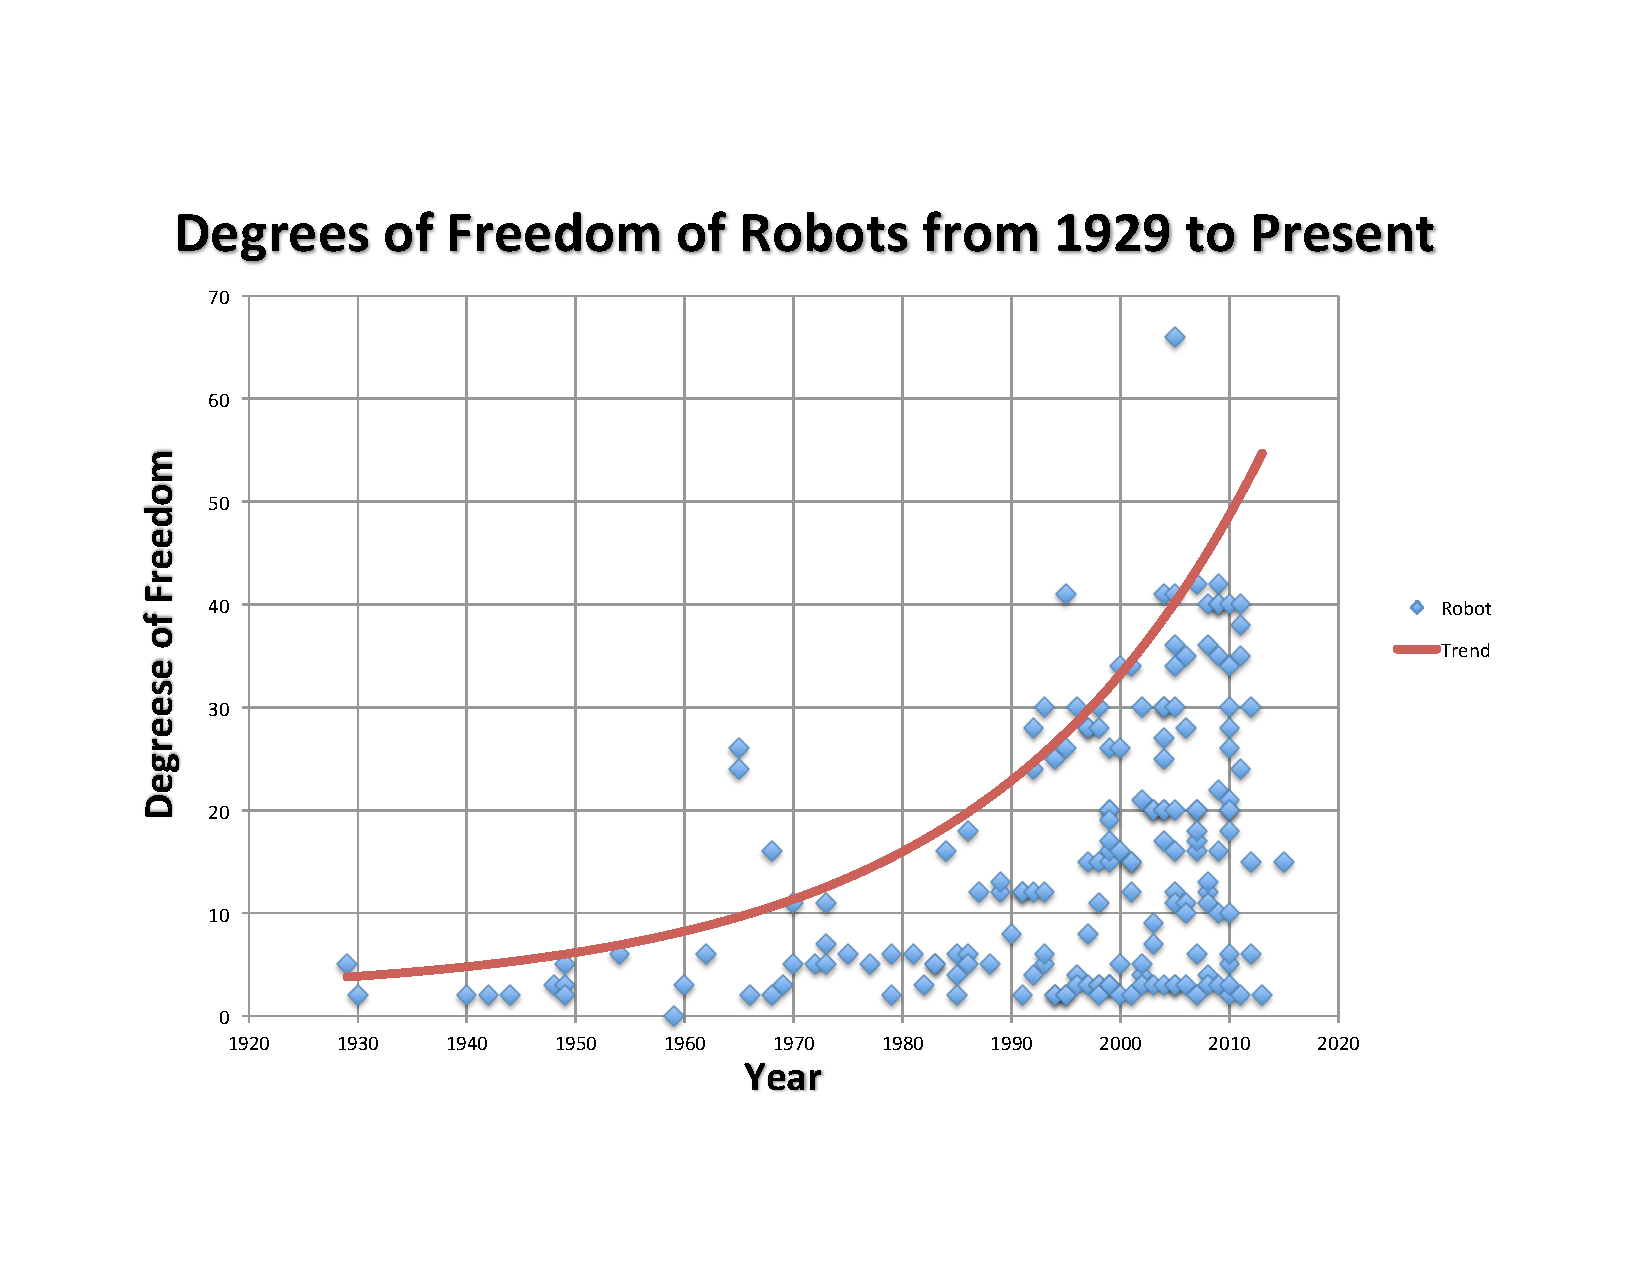
\includegraphics[width=0.8\columnwidth]{./pix/robotsDOF.pdf}
\caption{Number of degrees of freedom for robots form 1929 to the present.}
\label{fig:numOfRobots}
\end{figure}





It is common place for a complex electrical mechanical system to have multiple different controllers running in tandem.  
Different controllers are needed when the system is in different states or doing different tasks.
Combining these controllers is a problem in complex system.
This problem is hard when each controller has different frequencies, timing requirements (asyncronous vs. syncronous), latency restrictions, newest state data ie smore important then older state data and most basic of all languages the controller is written in.
This is especially true for complete and complex autonomous systems.
I define a complete and complex autonomous system as an electro mechanical mechanism with high degree of freedom (DOF) that is capable of making its own decisions through the use of sensor data processed by its artificial intelligence (AI).
The combination of high DOF and the requirement for autonomy makes the work space broad and controllers complex.
The overarching question becomes; What is the control system structure for a complete and complex autonomous systems with high DOF, a multitude of sensors, AI performing high-level and low-level tasks all while keeping a stable system structure conducive to collaborative work?
Current methods of solving the problem of controller synchrony and latest state data is to keep your critical control elements in the primary control loop.
Inter-process communication (IPC) and/or network sockets to communicate between the high level and low level processes even if written in different languages.
The majority of IPC have the problem of \textit{head of line} blocking (HOL) which means you must read the older data in a buffer before you read the newest data.
In the computer science field this is not a problem because all data being intact is typically desired.  
In the field of robotics and control the most recent state data is more important to a real-time control system to act on.
This thesis shows that by expanding on the idea of multi-process controllers connected to high-speed low-latency IPC you can create a \textit{robot layer} on a computer platform that will allow low-level controllers to run in separate processes while still allowing them access to the most recent data as the priority.
The new technical idea is the \textit{robot layer}, a control layer that allows external processes to run like normal and not deal with the specifics of the given robot system.
The robot system can be replaced by a simulated system without any of the processes needing to be modified or even know of the change.
This allows more mature controllers to be easily interfaced with this system without modifying control rates or timing.
This \textit{robot layer} must be:
\begin{itemize}
\item Have a IPC latency much less then that of the robot's inherent sampling period $t_{ipc}<<T_{r}$
\item Allow for command rates much slower then the inherent sampling period $T_{slow}>>T_{r}$
\item Allow for command rates much faster then the inherent sampling period $T_{fast}<<T_{r}$
\item Allow for arbitrary command rates.
\item Allow for real-time and non-real-time controllers to command actuators
\item Allow for all processes to have access to the newest data first
\item Allow for no more then one rt time step delay between command and robot actuator retrieval
\item Commanded such that it is for an arbitrary robotic actuator.
\item Triggering for process synchronization
\item Triggering for simulator synchronization and holding
\end{itemize}
We can succeed now not only because the bleeding edge technology allows for the fast enough communication between processes with access to the latest data.

Results are measured quantitatively and qualitatively.
Data showing proper loop rates, timings, controller implementation, simulation connections etc. show the viability of the system.
User survey shows methodology is sound, useful, and practical.





My Thesis shows is that a multi-process control structure coupled with the proper timing mechanisms is conducive to answering these questions.
It is shown with physical experiments and the creation of Hubo-Ach\cite{lofaroRAM2013}; a fully functional Sim-Time and Real-Time control system for complete and complex autonomous systems.

Through experimentation I prove my control system is a viable way of controlling complete and complex autonomous system and still be conducive to collaborative work.  
A road map of how my research has taken me to my thesis is shown in Section~\ref{sec:roadmap}.
As proof of viability I show the basic structure of my system \textit{Hubo-Ach} in Section~\ref{sec:hubo-ach}.  
I give step by step examples in Section~\ref{sec:simpleExamples}.
Section~\ref{sec:simulator} shows how we can move from real-time to using a simulated version of the platform in simulation time without having to change the controller.
Section~\ref{sec:task} describes the experiment which consists of making the robot preform an advanced task that pulls together visual, kinematic, path planning and other controllers together using this one system.
The techniques used stem from my contributions in Section~\ref{sec:contributions}.
Section~\ref{sec:results} shows the results of the experiment thus show the viability of the system.
Lastly Section~\ref{sec:conclusion} discusses the results of the work and the future of this system.

Before I continue it is important to note that my work has already been validated by my pears because:
\begin{itemize}
\item It was chosen to be the primary control system for the DARPA Robotics Challenge Track-A Team DRC-Hubo, Section~\ref{sec:drc}.
\item It is being used in the NSF-MIRR project\footnote{NSF-MIRR: Major Research Infrastructure Recovery and Reinvestment (MIRR) \#CNS-0960061 sponsored by the the U.S. National Science Foundation (NSF)}.
\item It is currently being used by MIT, WPI, Purdue, Ohio State, Swarthmore College, Georgia Tech, and Drexel University.
\end{itemize}

For the remainder of this document the complete and complex autonomous systems that I will be referring to are robots.
The majority of examples given will be in reference to humanoid robotics and the Hubo2+ (KHR-4+) platform.
The Hubo platform is described in Section~\ref{sec:hubo}.




